%!TEX root = ../final.tex
\question Researchers collected data on the number of times students have
stepped on a UC Berkeley seal in the past year and students’ GPAs. A
scatterplot of GPA on number of steps (left), as well as the table \code{seal}
(middle) and its corresponding statistics (right), is displayed below. You may
assume that statistics in that table are good approximations to their
corresponding population parameters.

\begin{figure}[h!]
\begin{floatrow}
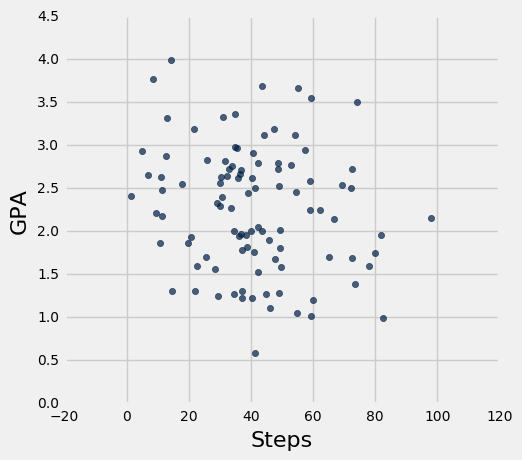
\includegraphics[width=0.18\textwidth]{figs/steps_and_gpa.png}
% \ffigbox{%
%   \rule{3cm}{3cm}%
% }{%
%   \caption{A figure}%
% }
\capbtabbox{%
  \begin{tabular}{|c|c|c|} \hline
  Student ID  & Steps   &  GPA \\ \hline
  25789012    &   65    &  2.86 \\ \hline
  38973744    &   39    &  3.76 \\ \hline
  31402938    &   96    &  3.12 \\ \hline
  \end{tabular}

  \code{... (97 rows omitted)}
}{}
\capbtabbox{%
  \begin{tabular}{|c|c|c|} \hline
  Statistic & Steps & GPA \\ \hline
  Mean      & 50    & 2.5 \\ \hline
  Std Dev   & 20    & 1.5 \\ \hline
  \end{tabular}
}{}
\end{floatrow}
\end{figure}

\begin{parts}

\part[4] Researchers want to create a confidence interval for the true slope of
the regression line predicting GPA given the number of steps on the seal.
Complete the code below so that the last line outputs a 90\% confidence
interval.

You may use the \code{slope(table, x\_label, y\_label)} function defined in
class which takes in a table, the label/index for the x-values, and the
label/index for the y-values, in that order. It returns the slope in original
units of the regression line predicting y given x.

\begin{verbatim}
slopes = make_array()
for i in np.arange(5000):

    resample = ___________________________________________________

    bootstrapped_slope = _________________________________________

    slopes = __________________ (slopes, _______________________ )

[percentile(________, slopes), percentile(________, slopes)]
\end{verbatim}

\begin{solution}
\begin{verbatim}
slopes = make_array()
for i in np.arange(5000):
    resample = seal.sample()
    bootstrapped_slope = slope(resample, "Steps", "GPA")
    slopes = np.append(slopes, bootstrapped_slope)

print(percentile(5, slopes), percentile(95, slopes))
\end{verbatim}
\end{solution}

\part[12] Assume the code above was implemented correctly and researchers
generate an interval of $(-0.25, 0.12)$ for the population regression slope.
Evaluate whether each statement is true or false and \textbf{briefly} justify
your answer.

\begin{subparts}
  \subpart Because the interval contains 0, for a p-value cutoff of
    5\% we fail to reject the null hypothesis that the slope of the population
    regression line is 0.

    \begin{oneparcheckboxes}
      \correctchoice True
      \choice False
    \end{oneparcheckboxes}

    \begin{solutionorbox}[0.8in]
      True. The confidence interval fails to reject this null hypothesis at a
      cutoff of 10\%, which means we would also fail to reject the null at a
      cutoff of 5\% (which gives a wider interval).
    \end{solutionorbox}

  \subpart If we rerun the code in part (a) 100 times, we expect that around 90
    of the intervals will contain the true population slope.

    \begin{oneparcheckboxes}
      \choice True
      \correctchoice False
    \end{oneparcheckboxes}

    \begin{solutionorbox}[0.8in]
      False. We aren't getting a new sample from the population, so if we reran
      the code in part (a) we would get approximately the same interval every
      time.
    \end{solutionorbox}

  \subpart The population regression slope falls within this interval about
    90\% of the time.

    \begin{oneparcheckboxes}
      \choice True
      \correctchoice False
    \end{oneparcheckboxes}

    \begin{solutionorbox}[0.8in]
      False. The population regression slope either falls within this
      interval or it doesn't.
    \end{solutionorbox}

  \subpart If we instead try to predict number of steps using GPA, we will
    still get roughly the same confidence interval endpoints.

    \begin{oneparcheckboxes}
      \choice True
      \correctchoice False
    \end{oneparcheckboxes}

    \begin{solutionorbox}[0.8in]
      False. Although the interval will likely contain 0, the units of the
      interval will be different so the endpoints will also be different.
    \end{solutionorbox}
\end{subparts}

\part[3] Suppose researchers are now interested in the average number of times
students have stepped on the UC Berkeley seal in the past year. What sample
size do they need to create a 95\% confidence interval such that the interval
width is 4 or less? If you need more information to solve this problem, state
what information you need.

\begin{solutionorbox}[1in]
The interval width must be 4 or less and there are 4 standard deviations in a
95\% confidence interval, so the standard deviation of the sample distribution
must be 1 or less. Using the sample standard deviation as an approximation for
the population standard deviation and applying the CLT, we get:

\begin{align*}
  \frac{20}{\sqrt{n}} &\leq 1 \\
  n &\geq 400
\end{align*}
\end{solutionorbox}

\checkboxchar{$\Box$}
\part[5] Using the data from \code{seal}, researchers create a 95\%
bootstrap confidence interval for the average number of times students have
stepped on a UC Berkeley seal in the past year. Which of the following
statements is/are true about this interval? Select all that apply.
\begin{checkboxes}
  \choice If researchers draw another sample and computed a second confidence
  interval, it will always overlap with the first interval.
  \choice If researchers increase their sample size from 100 to 1000, they will
  always get a smaller bootstrap confidence interval.
  \choice If the researchers increase their bootstrap resample size from 100 to
  1000, they will always get a confidence interval they can use to conduct a
  valid hypothesis test.
  \choice If the researchers increase their bootstrap repetitions from 5000 to
  10000, they can expect their confidence interval to be narrower.
  \correctchoice If the researchers resampled without replacement, the
  resulting interval will always have a width of 0.
\end{checkboxes}

\begin{solution}
  Choice 1 is false. We are not guaranteed that the intervals will overlap
  since we could get a sample that looks completely different from our first
  one.

  Choice 2 is false. We are not guaranteed that the new interval will be
  smaller, although it is highly likely.

  Choice 3 is false. We must resample the same number of items as the original
  sample for our confidence interval to be valid.

  Choice 4 is false. Increasing the bootstrap repetitions makes the empirical
  distribution of the test statistic smoother but does not significantly change
  the boundaries of the confidence interval.

  Choice 5 is true. If we resample without replacement, we will get the same
  resampled slope every time.
\end{solution}

\part[4] Which of the following statements are true about the confidence
interval created in part (a) and the confidence interval in part (d)? Select
all that apply.
\begin{checkboxes}
  \correctchoice Neither interval is guaranteed to contain the parameter it is trying to estimate.
  \choice The interval in part (d) will be wider because it has a higher
  confidence level.
  \choice The two intervals used different resample sizes.
  \choice The interval estimating the population regression slope can be used
  to test a null hypothesis, but the one estimating average steps on the seal
  cannot.
\end{checkboxes}

\begin{solution}
  Choice 1 is true. We are not guaranteed that either interval will contain
  the parameter.

  Choice 2 is false. The interval in (d) will be wider because it has
  different units, not because of its confidence level.

  Choice 3 is false. We must resample the same number of items as the original
  sample for both confidence intervals.

  Choice 4 is false. Both intervals can be used for hypothesis testing.
\end{solution}

\end{parts}
